% !TeX program = PdfLaTeX
% !TeX root = ../../Elaborati_Aerodinamica_Bruno_Spoti.tex

\chapter{Il carico lungo l'ala}
In questo capitolo saranno applicate diverse metodologie per il calcolo del carico lungo l'ala e della distribuzione del coefficiente di portanza. In primo luogo è stato utilizzato il metodo di Schrenk, rendendo preliminarmente la forma in pianta diritta, essendo il velivolo scelto dotato di freccia. Successivamente sono stati corretti i risultati ottenuti tramite il metodo di Schrenk applicando un'estensione del metodo alle ali a freccia, proposta da Pope \& Haney.\\
Tutti i calcoli sono stati effettuati utilizzando una routine appositamente realizzata in Matlab, che assegnata una geometria in input, permette di calcolare la distribuzione delle grandezze geometriche e aerodinamiche lungo la semi apertura, l'ala ellittica equivalente, facendo un controllo sulle aree, il carico addizionale secondo il metodo di Schrenk, il carico basico, la distribuzione di coefficiente di portanza, e la correzione di Pope \& Haney.

\section{Il metodo di Schrenk}

Il metodo ingegneristico di Schrenk è un metodo semiempirico che consente il calcolo del carico aerodinamico lungo un'ala dritta nell’ipotesi di assenza di fenomeni viscosi a basse velocità. Tale metodo ha il vantaggio di consentire una valutazione piuttosto veloce ed accettabilmente accurata del carico, molto utile in sede di progetto preliminare.\\
L'ipotesi alla base del metodo di Schrenk consiste nel valutare il carico addizionale lungo l'apertura, come media tra la distribuzione delle corde effettive dell'ala in esame e la distribuzione delle corde di un'ala ellittica avente la stessa area in pianta e la stessa apertura.
In primo luogo sarà ricavato il carico addizionale lungo la semiala, e in seguito verrà valutato anche il carico basico al fine di ottenere il carico totale lungo l’ala. \\ Le analisi saranno condotte sull'ala in figura~\vref{fig:V3}, i cui dati sono riportati in tabella~\vref{tabV1}. 

\begin {figure} [H]
\centering
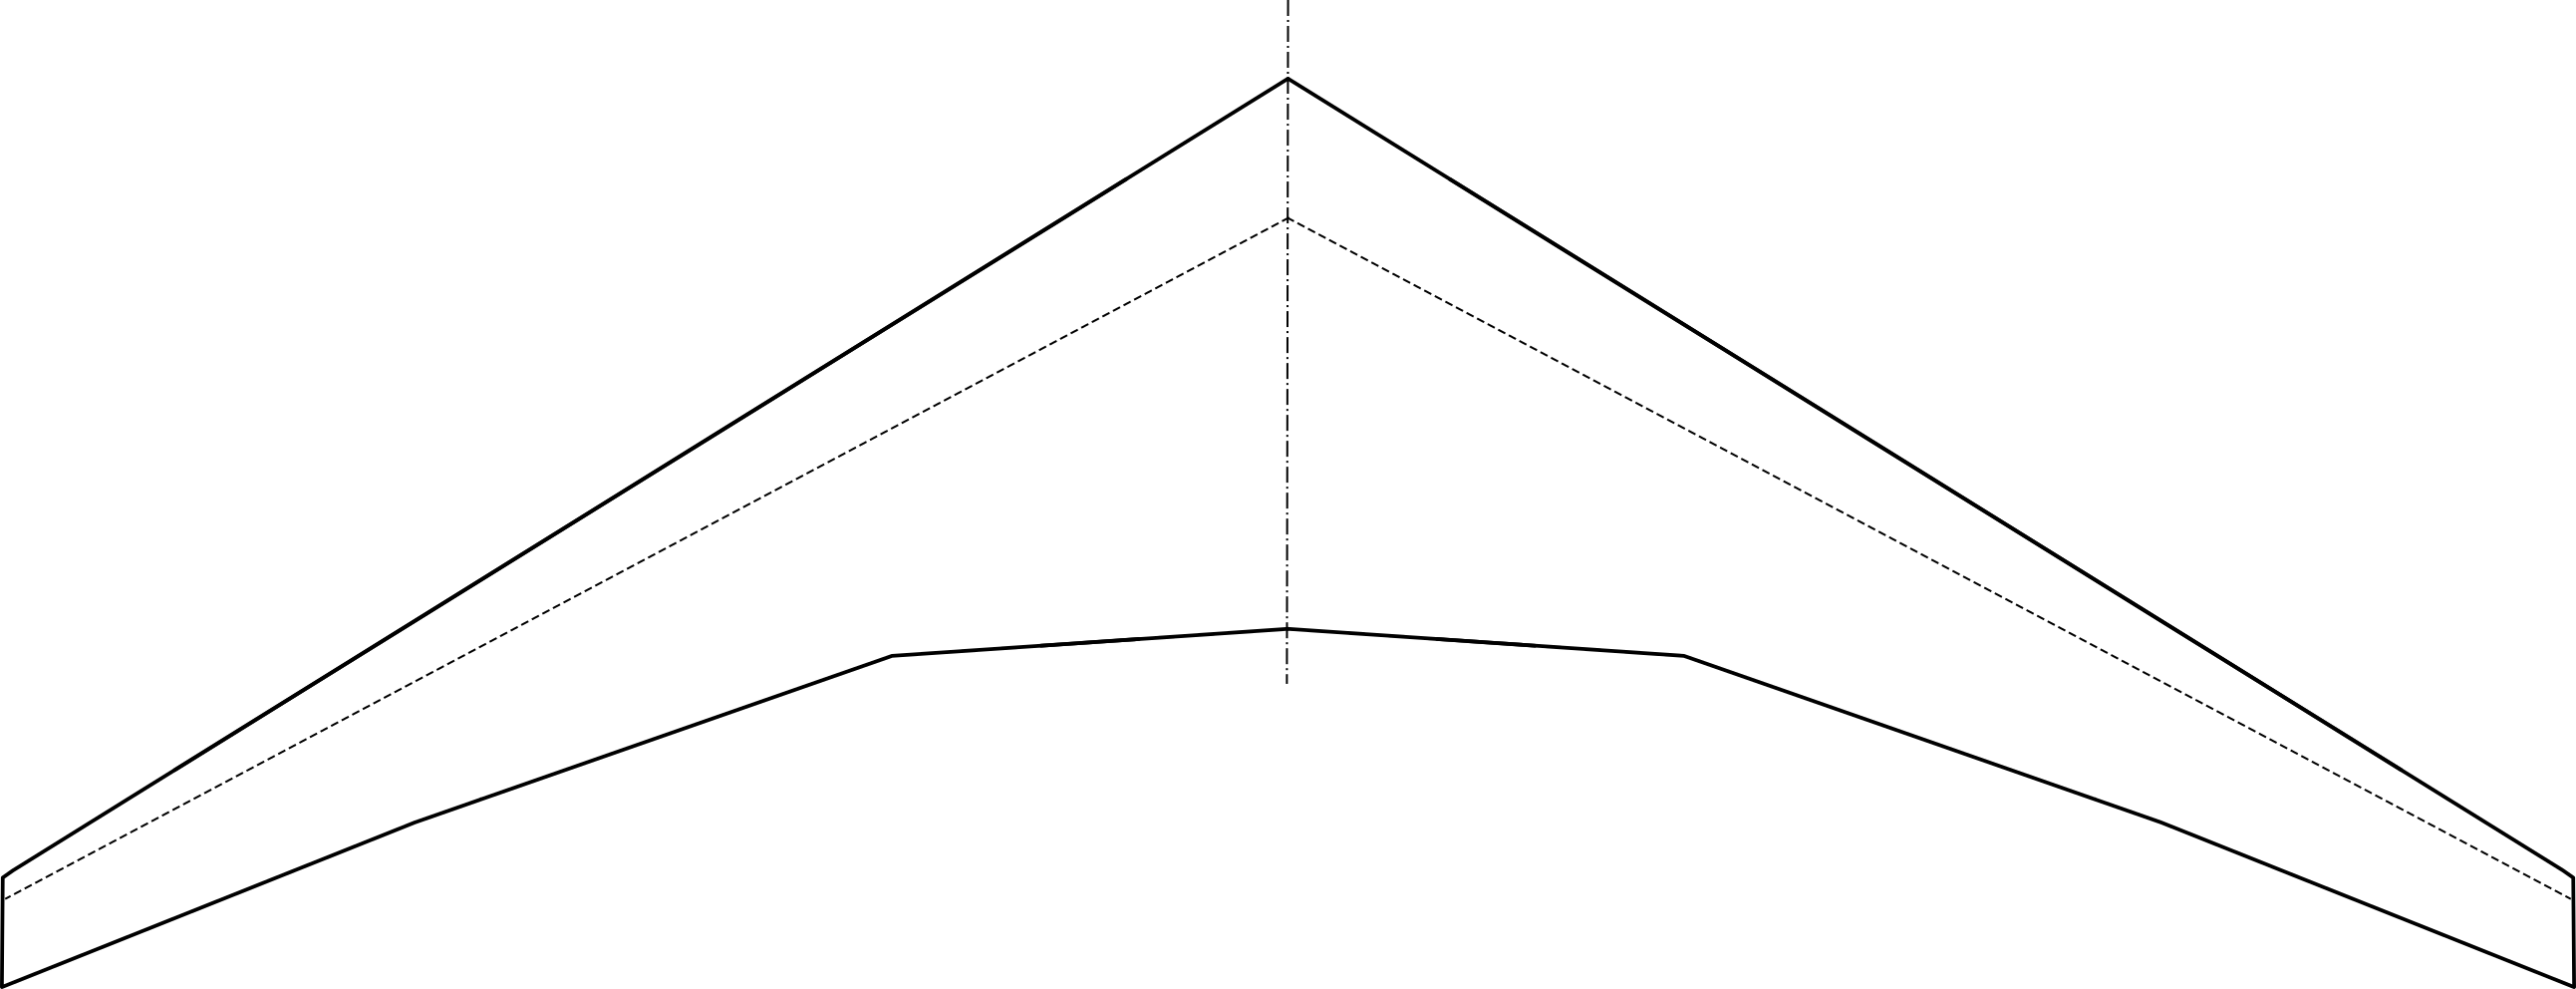
\includegraphics[width= \textwidth ]{images/fileImg/Parte_3-Aerodinamica_Velivolo_A340-200/AlaA340_200_nowl.png}
\caption{\footnotesize Forma in pianta dell'ala dell' Airbus A340-200, configurazione senza winglet.}
\label {fig:V3}
\end {figure}
\begin{figure}[h!]
	\centering
	\begin{tikzpicture}
	\begin{axis}[ 
	xmin=0, 
	xmax=1, 
	ymin=0, ymax=14,
	xlabel=$ \eta$, 
	ylabel=c (m),
	ylabel style={rotate=-90},
	width=13cm,
	height=8cm,
	scale only axis,
	grid=major] 
	\addplot [black,solid]
	file{images/fileDat/Parte_3-Aerodinamica_Velivolo_A340-200/Schrenk/c_vs_eta.dat};
	\addplot [black,solid, thin]
	file{images/fileDat/Parte_3-Aerodinamica_Velivolo_A340-200/Schrenk/c_ell_vs_eta.dat};
	\addplot [black,solid,dashed]
	file{images/fileDat/Parte_3-Aerodinamica_Velivolo_A340-200/Schrenk/c_mean_vs_eta.dat};
	\legend {Distribuzione di corde, Distribuzione di corde dell'ala ellittica, Media}
	\end{axis}
	\end{tikzpicture}
	\caption{\footnotesize Velivolo Airbus A340-200. Confronto tra la distribuzione di corde e la distribuzione di corde di un'ala ellittica equivalente. MATLAB R2016b. }
	\label{fig:V4}
\end{figure}

La correttezza del risultato è stata verificata tramite un confronto delle aree dell'ala dell' Airbus A340-200 e l'ala ellttica equivalente, come riportato in figura~\vref{tabV4}.

\begin{table} [!h]\centering \rowcolors{1}{}{grigio_chiaro}
	\begin{tabular}{c c }
		\toprule
		\emph{Geometria fornita }& \emph{Ala ellittica equivalente}\\ 
		\midrule
		S = 370,444 \si{m^2} &	S = 370,440 \si{m^2}\\
		\bottomrule
	\end{tabular}
	\caption {\footnotesize Velivolo A340-200. Confronto tra le superfici alari della geometria fornita e dell'ala ellittica equivalente.}
	\label{tabV4}
\end{table}

\begin{figure}[H]
	\centering
	\begin{tikzpicture}
	\begin{axis}[ 
	xmin=0, 
	xmax=1, 
	ymin=0, ymax=0.1,
	xlabel=$ \eta$, 
	ylabel=$\gamma$,
	ylabel style={rotate=-90},
	width=13cm,
	height=7cm,
	scale only axis,
	grid=major] 
	\addplot [black,solid]
	file{images/fileDat/Parte_3-Aerodinamica_Velivolo_A340-200/Schrenk/gamma_a1_vs_eta.dat};
	\end{axis}
	\end{tikzpicture}
	\caption{\footnotesize Velivolo Airbus A340-200. Carico addizionale calcolato con il metodo di Schrenk per $C_L=1$. MATLAB R2016b. }
	\label{fig:V5}
\end{figure}


\begin{figure}[H]
	\centering
	\begin{tikzpicture}
	\begin{axis}[ 
	xmin=0, 
	xmax=1, 
	ymin=0, ymax=1.5,
	xlabel=$ \eta$, 
	ylabel=$C_l$,
	ylabel style={rotate=-90},
	width=13cm,
	height=7cm,
	scale only axis,
	grid=major] 
	\addplot [black,solid, thick]
	file{images/fileDat/Parte_3-Aerodinamica_Velivolo_A340-200/Schrenk/Cl_CL_1_vs_eta.dat};
	\addplot [black,solid, thin]
	file{images/fileDat/Parte_3-Aerodinamica_Velivolo_A340-200/Schrenk/Cl_CL_04_vs_eta.dat};
	\legend{$C_L=1$, $C_L=0.4$}
	\end{axis}
	\end{tikzpicture}
	\caption{\footnotesize Velivolo Airbus A340-200. Distribuzione di $C_l$ calcolato con il metodo di Schrenk, a diversi coefficienti di portanza dell'ala. MATLAB R2016b. }
	\label{fig:V6}
\end{figure}

Il carico basico, dovuto allo svergolamento, si considera proporzionale alla metà dello svergolamento realmente esistente

\begin{equation}
\label{eqn:bas}
cC_{l_b}=cC_{l_{\alpha}} \frac{1}{2}(\varepsilon_y-[\alpha]_{C_L=0})
\end{equation}

I profili utilizzati per l’ala sono profili supercritici, con spessore costante fino alla stazione del {\itshape kink}, riportati nella tabella 

\begin{table} [!h]\centering \rowcolors{1}{}{grigio_chiaro}
	\begin{tabular}{c  c  c c c }
		\toprule
		\emph{Stazione}& \emph{Profilo}&\alphazl & $C_{l_{\alpha}}$& $\varepsilon$ \\ 
		\midrule
		{\itshape Root}, {\itshape Kink}	&	SC(2)-0610	&	$-3.82 ^{\circ}$	& $6.64 {\mathrm rad}^{-1}$	&$0^{\circ}$	\\
		{\itshape Tip} &  SC(2)-0614 &	$-3.57 ^{\circ}$	& $6.56 {\mathrm rad}^{-1}$	&	$-4^{\circ}$	\\
		\bottomrule
	\end{tabular}
	\caption {\footnotesize Velivolo A340-200. Profili lungo l'apertura}
	\label{tabV3}
\end{table}

Al fine di poter calcolare il carico basico, si suppone uno svergolamento di $-4^\circ $ all' estremità e svergolamento nullo alla radice e {\itshape kink}, con una legge di variazione lineare. L’angolo di portanza nulla dell’ala risulta essere $ \alpha_{ZL}=-2.2^\circ$

\begin{figure}[h!]
	\centering
	\begin{tikzpicture}
	\begin{axis}[ 
	xmin=0, 
	xmax=1, 
	ymin=-0.5, ymax=2,
	xlabel=$ \eta$, 
	ylabel=$C_l$,
	ylabel style={rotate=-90},
	width=13cm,
	height=7cm,
	scale only axis,
	grid=major] 
	\addplot [black,solid, thin]
	file{images/fileDat/Parte_3-Aerodinamica_Velivolo_A340-200/Schrenk/Cl_CL_1_vs_eta.dat};
	\addplot [black,solid,thin, dashed]
	file{images/fileDat/Parte_3-Aerodinamica_Velivolo_A340-200/Schrenk/Cl_b.dat};
	\addplot [black,solid, very thick]
	file{images/fileDat/Parte_3-Aerodinamica_Velivolo_A340-200/Schrenk/Cl_tot.dat};
	\legend{$C_l$ addizionale, $C_l$ basico,$C_l$ totale}
	\end{axis}
	\end{tikzpicture}
	\caption{\footnotesize Velivolo Airbus A340-200. Distribuzione di $C_l$ basico e addizionale e totale per $C_L = 1$. MATLAB R2016b. }
	\label{fig:V6}
\end{figure}


\section{Carico alare effettivo secondo Pope \& Haney}
Un’estensione del metodo di Schrenk alle ali a freccia, proposta da Pope ed Haney, permette di correggere i risultati ottenuti dal metodo di Schrenk introducendo un fattore proporzionale al coseno della freccia. L'effetto della freccia è quello di ridurre il $C_L$ dell'ala, pertanto il confronto tra i due metodi è stato fatto a parità di $C_L$, scalando quello ottenuto dal metodo Pope \& Haney.
Come si può notare dalla figura~\vref{fig:V8} a pari coefficiente di portanza, la freccia sposta i carichi verso l’esterno se positiva, effetto visibile nonostante lo svergolamento d'estremità. 

\begin{figure}[h!]
	\centering
	\begin{tikzpicture}
	\begin{axis}[ 
	xmin=0, 
	xmax=1,  
	ymin=0, ymax=1.6,
	xlabel=$ \eta$, 
	ylabel=$C_l$,
	ylabel style={rotate=-90},
	width=13cm,
	height=7cm,
	scale only axis,
	grid=major] 
	\addplot [black,solid, very thick]
	file{images/fileDat/Parte_3-Aerodinamica_Velivolo_A340-200/Schrenk/Cl_CL_1_vs_eta.dat};
	\addplot [black,solid, thin]
	file{images/fileDat/Parte_3-Aerodinamica_Velivolo_A340-200/Schrenk/Cl_sweep_correct_vs_eta.dat};
	\legend{Metodo di Schrenk , Correzione Pope \& Haney}
	\end{axis}
	\end{tikzpicture}
	\caption{\footnotesize Velivolo Airbus A340-200. Distribuzione di $C_l$ calcolato con il metodo di Schrenk, e correzione Pope \& Haney, per $C_L=1$. MATLAB R2016b. }
	\label{fig:V8}
\end{figure}

\begin{figure}[h!]
	\centering
	\begin{tikzpicture}
	\begin{axis}[ 
	xmin=0, 
	xmax=1, 
	ymin=0, ymax=0.1,
	xlabel=$ \eta$, 
	ylabel=$\gamma$,
	ylabel style={rotate=-90},
	width=13cm,
	height=7cm,
	scale only axis,
	grid=major] 
	\addplot [black,solid]
	file{images/fileDat/Parte_3-Aerodinamica_Velivolo_A340-200/Schrenk/gamma_a1_vs_eta.dat};
	\addplot [black,solid, thin]
	file{images/fileDat/Parte_3-Aerodinamica_Velivolo_A340-200/Schrenk/gamma_sweep_vs_eta.dat};
	\legend{Metodo di Schrenk , Correzione Pope \& Haney}
	\end{axis}
	\end{tikzpicture}
	\caption{\footnotesize Velivolo Airbus A340-200.Distribuzione del carico alare calcolato con il metodo di Schrenk, e correzione Pope \& Haney, per $C_L=1$. MATLAB R2016b. }
	\label{fig:V7}
\end{figure}

